%! Author = wolfram_e_laube
%! Date = 16.04.24

\item[(d)]
To verify the correct implementation of the convolution, the output is compared with the result obtained using Python's built-in \texttt{numpy.convolve} function. The following Python script performs this comparison and plots both signals:

\begin{verbatim}
import numpy as np
import matplotlib.pyplot as plt

# Calculate the convolution using numpy's built-in function
y_conv = np.convolve(x, h, mode='full')

# Plot both signals for comparison
plt.figure(figsize=(12, 6))
plt.stem(np.arange(len(y)), y, linefmt='b-', markerfmt='bo', basefmt='b-', label='Manual Convolution', use_line_collection=True)
plt.stem(np.arange(len(y_conv)), y_conv, linefmt='r--', markerfmt='ro', basefmt='r--', label='Numpy convolve', use_line_collection=True)
plt.title('Comparison of Manual and Numpy Convolution')
plt.xlabel('Sample index $n$')
plt.ylabel('Amplitude')
plt.legend()
plt.grid(True)
plt.show()
\end{verbatim}

This verification confirms the accuracy of the manual convolution method by visually comparing it against the convolution computed by \texttt{numpy.convolve}. Different line styles and colors are used in the plot to clearly differentiate between the two results.

\begin{figure}[h]
\centering
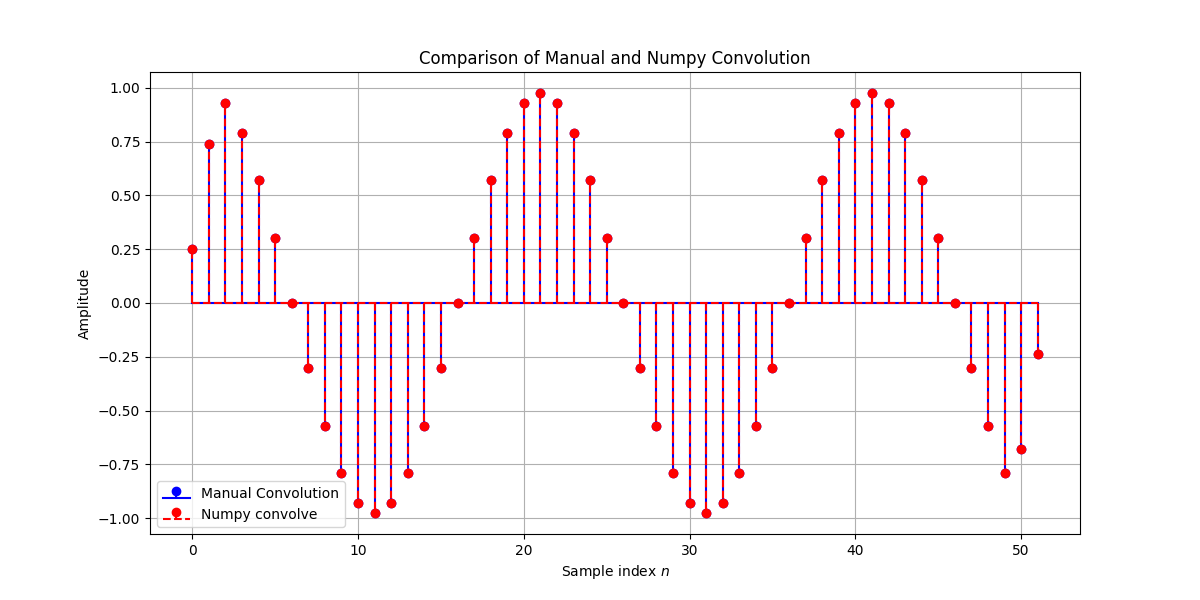
\includegraphics[width=\textwidth]{fig/ex3_plot_2}
\caption{The requested plot}
\label{fig:ex3_plot_2}
\end{figure}
